\documentclass{homework}
\usepackage{enumitem}
\usepackage{tikz}
\usepackage{diagbox}
\usetikzlibrary{positioning,shapes,arrows}

\title{Assignment9: Learning}
\author{
  \texttt{<xiangru.chen@fau.de>} \\
  \texttt{yd08ucoz}
  \and
 \texttt{<yamei.zhao@fau.de>}\\
  \texttt{mo02buqo}
  \and
  \texttt{<ekaterina.bobrova@fau.de>}\\
  \texttt{il71ywod}
}
\begin{document}

\maketitle

\exercise[9.1 (Statistical Learning)]
We use two observations to determine if it has rained on our property: whether the ground is wet, and whether a bucket we left outside is full.
\begin{enumerate}
	\item Model this situation as a naive Bayesian network with a boolean class and two boolean attributes.
		\begin{center}
		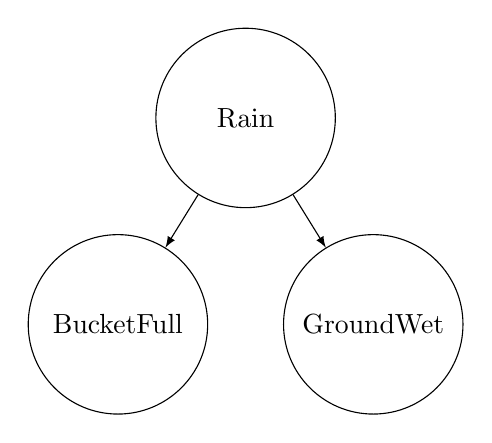
\begin{tikzpicture}[
		  node distance=1cm and 0cm,
		  mynode/.style={draw,circle,text width=2cm,align=center}
		]
		\node[mynode] (Rain) {Rain};
		\node[mynode, below right=of Rain] (GroundWet) {GroundWet};
		\node[mynode,below left=of Rain] (BucketFull) {BucketFull};
		\path (Rain) edge[-latex] (GroundWet)
			(Rain) edge[-latex] (BucketFull);
		\end{tikzpicture}
		\end{center}
	\item Explain why this network requires 5 parameters (2n + 1 where n = 2 is the number of attributes). Choose 5 names for the parameters and use them to give the conditional probability table of the network.

	For each node that has a parent conditional probabilities are required depending on the value of the parent node.  Also, distributions of parents nodes are also required. Since there are 2 children nodes and 1 parent node and dimension of each node is 2,  this network requires 5 conditional probabilities(i.e. parameters).

	Let $\theta_R = P(R=yes), \theta_{BF|R} = P(BF=yes|R=yes),\theta_{BF|\lnot R} = P(BF=yes|R=no), \newline\theta_{GW|R} = P(GW=yes|R=yes), \theta_{GW|\lnot R} = P(GW=yes|R=no)$, where GW - GroundWet, BF - BucketFull.

\item State the formula for the likelihood of this list of 50 observations in terms of the 5 parameters.

$P(R|\theta_R, \theta_{BF|R}, \theta_{BF|\lnot R},\theta_{GW|R},\theta_{GW|\lnot R})=\theta_R^{\# R}(1-\theta_R)^{\# \lnot R}\cdot \theta_{BF|R}^{\# BF|R}(1-\theta_{BF|R})^{\# \lnot BF|R}\cdot\newline \theta_{BF|\lnot R}^{\# BF|\lnot R}(1-\theta_{BF|\lnot R})^{\# \lnot BF|\lnot R}\cdot \theta_{GW|R}^{\# GW|R}(1-\theta_{GW|R})^{\# \lnot GW|R}\cdot \theta_{GW|\lnot R}^{\# GW|\lnot R}(1-\theta_{GW|\lnot R})^{\# \lnot GW|\lnot R}$
\item Give the Maximum Likelihood approximations for the 5 parameters given these 50 observations.

$\theta_R = \dfrac{\# R}{\# R + \# \lnot R}=\dfrac{25}{50}=\dfrac{1}{2},\theta_{BF|R} = \dfrac{\# BF|R}{\# BF|R + \# \lnot BF|R}=\dfrac{16}{25},\newline\theta_{BF|\lnot R} = \dfrac{\# BF|\lnot R}{\# BF|\lnot R + \# \lnot BF|\lnot R}=\dfrac{5}{25}=\dfrac{1}{5},\theta_{GW|R} = \dfrac{\# GW|R}{\# GW|R + \# \lnot GW|R}=\dfrac{15}{25}=\dfrac{3}{5},\newline\theta_{GW|\lnot R} = \dfrac{\# GW|\lnot R}{\# GW|\lnot R + \# \lnot GW|\lnot R}=\dfrac{11}{25}$
\end{enumerate}


\end{document}